
\chapter{Introduzione}


La crittografia è un metodo per un utente di condividere in maniera sicura i propri dati su un mezzo di comunicazione o un sito insicuri.\\
Prima della crittografia a chiave pubblica, un metodo ampiamente utilizzato tra due utenti per comunicare informazioni confidenziale era quello di stabilire a priori un segreto comune e ben protetto che permettesse di decodificare le informazioni.\\
Nonostante questo metodo possa esser accettabile per piccoli gruppi diventa obsoleto ed inutilizzabile in una infrastuttura molto grande come quella di Internet che conta miliardi di utenti.\\

Quasi 40 anni fa, Diffie ed Hellman pubblicarono una rivoluzionaria idea racchiusa nel concetto di \textbf{crittografia a chiave pubblica}:\\
{ \itshape ``due gruppi possono comunicare in maniera sicura \emph{senza} dover accordarsi su un segreto comune.''}

\vspace{0.4cm}

Al giorno d'oggi la crittografia a chiave pubblica è uno strumento fondamentale e il suo utilizzo è centrale per la communicazione sicura via web, alla cifratura di dispositivi d'archiviazione e per la possibilità di garantire l'autenticità di persone mediante firma digitale.


Vi sono delle particolarità per questa tipologia di crittografia:
\begin{itemize}
	\item Crittare è un metodo per inviare un messggio ad \textbf{una singola} entità che detiene una chiave segreta
	\item L'accesso ai dati cifrati è totale o nulla : una persona può decifrare e leggere completamente il messaggio \textbf{o} non può nemmeno decifrarlo.
\end{itemize}

\vspace{1cm}
Siamo interessati a risolvere un problema formulabile come:

\begin{center}
{\itshape È possibile costruire un sistema crittografico dove sia possibile crittare \textbf{una} volta sola il messaggio per poi distribuirla a più persone creando la possibilità di filtrare il contenuto in base alla persona che cerca di decifrarla?}
\end{center}
\newpage

Se dovessimo utilizzare la normale assunzione DH con chiavi pubbliche, avremo ad esempio un sistema di questo tipo:

\begin{center}
\begin{minipage}[c]{0.9\textwidth}
		\centering
		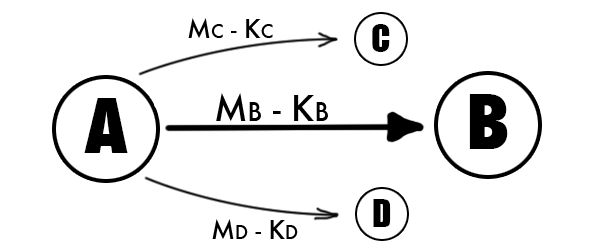
\includegraphics[keepaspectratio,width=\textwidth]{keying.png}\\
		{\small\scshape Un messaggio $M$ deve esser criptato con la chiave $K_I$ per esser mandata all'utente $I$}
\end{minipage}
\end{center}

Dove siamo costretti ad avere molte chiavi diverse per permettere la comunicazione verso ogni destinatario. Il messaggio viene crittato tante volte quanti sono i destinatari.\\[0.3cm]

Per questo motivo, Sahai and Waters \cite{sahai} fanno i primi passi per risolvere il problema intriducendo il concetto di ABE : Attribute Based Encryption.\\
Questo schema prevede la definizione di un insieme di attributi che funzioneranno da \emph{etichettatura} per ogni messaggio crittato.\\
La chiave di decifratura verrà calcolata per ogni utente in base ad una combinazione logica di attributi ben precisa: viene così creata una vera e propria policy d'accesso differenziata per ogni utente.\\[0.4cm]
A questo punto, l'utente è in grado di crittare il messaggio \emph{attaccandogli} gli attributi che preferisce. Questi attributi definiranno quali utenti potranno decifrare il messaggio: le chiavi che rispettano la policy, utilizzando gli attributi del messaggio, hanno diritto e possono decrittarlo.\\[0.2cm]

\begin{center}
\begin{minipage}[c]{0.9\textwidth}
		\centering
		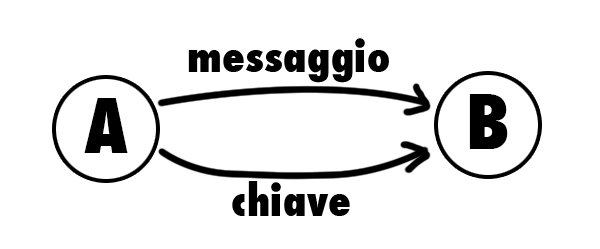
\includegraphics[keepaspectratio,width=\textwidth]{pairing.png}\\
		{\small\scshape Un unico messaggio etichettato con gli attributi viene mandato a tutti gli utenti. Solo gli utenti che detengono una chiave adatta possono leggere il messaggio.}
\end{minipage}
\end{center}

\newpage

La nascità e lo sviluppo dei servizi \emph{cloud} sono focalizzati sul problema iniziale, difficilmente risolvibile dalla crittografia a chiave publica.\\
Consideriamo un esempio concreto: \\
{\itshape un servizio di memorizzazione in cloud che immagazzina immagini per i diversi utenti registrati.\\
Le forze dell'ordine potrebbero aver bisogno di cercare sul cloud un immagine contenente un particolare volto.\\
Il gestore del servizio di cloud ha bisogno di fornire una chiave segreta alle forze dell'ordne che sia in grado di decifrare le immagini che contengono la faccia cercata ma che \textbf{non} visualizzi il resto delle immagini per non compromettere la privacy degli utenti non indagati.}\\[0.1cm]


Data la necessità di creare sistemi di crittografia che rispondessero a queste esigenze, vi sono stati molti tentativi diversi di costruzione matematica che rispondesse alle esigenze. \\
Lo strumento principale tra tutte queste costruzioni è un pairing $e$ tra gruppi ciclici. Questo pairing deve avere proprietà particolari (vedi \ref{pairinge}).\\
Esistono pairing complessi \cite{maas} \cite{benoit} tra cui il pairing di Tate e il pairing di Weil.\\[0.2cm]
Nello studio di questa tesi, sono stati evidenziati due diverse metodologie di crittografia:
\begin{itemize}
	\item \textbf{Identity Based Encryption} : Un garante genera per ogni utente delle chiavi private che vengono concesse unicamente se l'utente viene autenticato. A questo punto ogni utente autenticato avrà una propria chiave privata e pubblica dove questa seconda sarà possibile calcolarla on-the-fly utilizzando una \emph{frase caratteristica} come il numero di telefono o un indirizzo email. Con queste chiavi è possibile comunicare firmare e crittare i messaggi per poter esser communicati.\\
	Questo metodo, ideato temporalmente prima degli altri, è molto problematico e risente di difficoltà pratiche che lo rendono inutilizzabile per un applicazione reale.
	\item \textbf{Attribute Based Encryption} : Il sistema conosce a priori \emph{quanti} attributi gestirà. Da questi vengono create delle chiavi pubbliche che sono l'insieme di \emph{sottochiavi} per ogni singolo attributo. In questo modo ogni messaggio che viene cifrato, subisce una trasformazione \emph{neutra} rispetto agli attributi quando questi diventeranno fondamentali per decretare o meno l'autorizzazione della chiave per decifrare.
\end{itemize}

Nella prima tipologia, l'identità di una persona definisce la chiave rendendo il modello molto simile alla crittografia a chiave pubblica con la capacità di risolvere il problema principale seppur con qualche problema pratico: quando l'utente ha bisogno di rinnovare la propria coppia di chiavi e quella pubblica non può esser trovata da altre persone utilizzando la frase caratteristica originale poiché essa fornisce la vecchia chiave pubblica.\\
Nel secondo, gli attributi non definiscono chiavi ma bensì delle policy d'accesso. In questo modo chiavi e attributi si separano concettualmente risolvendo il problema.

\newpage

Altre differenze dettagliate sulla differenza dei due schemi si può trovare in \ref{ibeabe}\\[0.2cm]

Questo schema crittografico non è ancora pienamente conosciuto ed è per questo difficile definire e garantire un livello di sicurezza adatto per poter esser utilizzato nella quotidianità, come spiegato in \ref{secur}.\\[0.2cm]

In questa tesi verrà studiato lo schema ABE descritto in \cite{kpabe} nel seguente modo:
\begin{itemize}
	\item \textbf{Analisi del problema} e definizione astratta degli algoritmi utilizzati e della struttura d'accesso che vogliamo utilizzare.\\
	Definizione dell'algoritmo d'attacco per la definizione dell' assunzione decisionale bilineare di Diffie-Hellman.
	\item \textbf{Costruzione della struttura} d'albero e definizione analitica dei vari algoritmi. Effettiva costruzione dello schema crittografico e dimostrazione della sua correttezza d'utilizzo.
	\item \textbf{Dimostrazione dell'assunzione Diffie-Hellman}
\end{itemize}
\vspace{0.4cm}

Successivamente è presente un capitolo in cui vengono esposti gli strumenti utilizzati per la costruzione di un esempio con commenti comparativi con strutture e mappe più complesse. È stato anche brevemente discusso in \ref{security} un possibile schema d'attacco con un relativo commento sulla complessità che comporta lo schema studiato.\\[0.2cm]

Nell'ultimo capitolo sono stati aggiunti dei commenti sull'efficenza e sulla sicurezza del metodo per poi confrontarlo con altri schemi trovati.


